\subsection{First Isomorphism Theorem}
\begin{frame}
	\frametitle{First Isomorphism Theorem}
	\begin{theorem}
		Let $\phi : G \to G'$ be a group homomorphism with kernel $K$.
		And let $\gamma_K : G \to G/K$ be the canonical homomorphism.
		Then there is a unique isomorphism $\mu : G/K \to \phi[G]$
		such that $\phi(x) = \mu(\gamma_K(x))$.
	\end{theorem}
	\begin{figure}
	\centering
	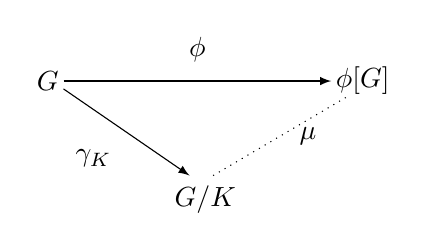
\begin{tikzpicture}
		\draw (0,1.5) node {$G$};
		\draw (2,0) node {$G/K$};
		\draw (4,1.5) node {$\phi[G]$};
		\draw[-latex] (0.2,1.4) -- node(e1)[sloped,label=below:$\gamma_K$]{} (1.8,0.3);
		\draw[-latex] (0.2,1.5) -- node(e2)[label=above:$\phi$]{} (3.6,1.5);
		\draw[dotted] (2.1,0.3) -- node(e2)[label=right:$\mu$]{} (3.8,1.3);
	\end{tikzpicture}
	\caption{First Isomorphism Theorem}
\end{figure}
\end{frame}
